\chapter{Classification of News Comments}
\label{ch:approach}

Our contribution is two-fold: First, we present a preprocessing technique to capture the conversation of a comment for classification.
Second, we adapt ULMFIT for German by training a German language model and publish it for further usage.

\section{Conversation-aware Classification of News Comments}
To exploit the sequential structure of news comment, we propose the preprocessing technique \textit{Prepend Previous} for language-model-based text classification.
News comments appear as part of a conversation where the news article acts as conversation starter.
Only considering each comment in isolation makes it hard to capture its true meaning.
Prepend Previous helps to overcome this restriction.
We prepend previous comments or parts of the article to each comment.
This is similar to the idea of Kochkina et al.~\cite{kochkina2017turing} for Branch-LSTM.
But they use use only word embeddings to represent text.
We use a recent way of using language models for representing text.
And since modern language models can capture dependencies over long distances, the content of a comment can be put into the context of the whole conversation.

\begin{figure}
    \centering
    \subfloat[<t><c>\textbf{1}</c><c>\textbf{2}</c><c>\textbf{3}</c></t>]{{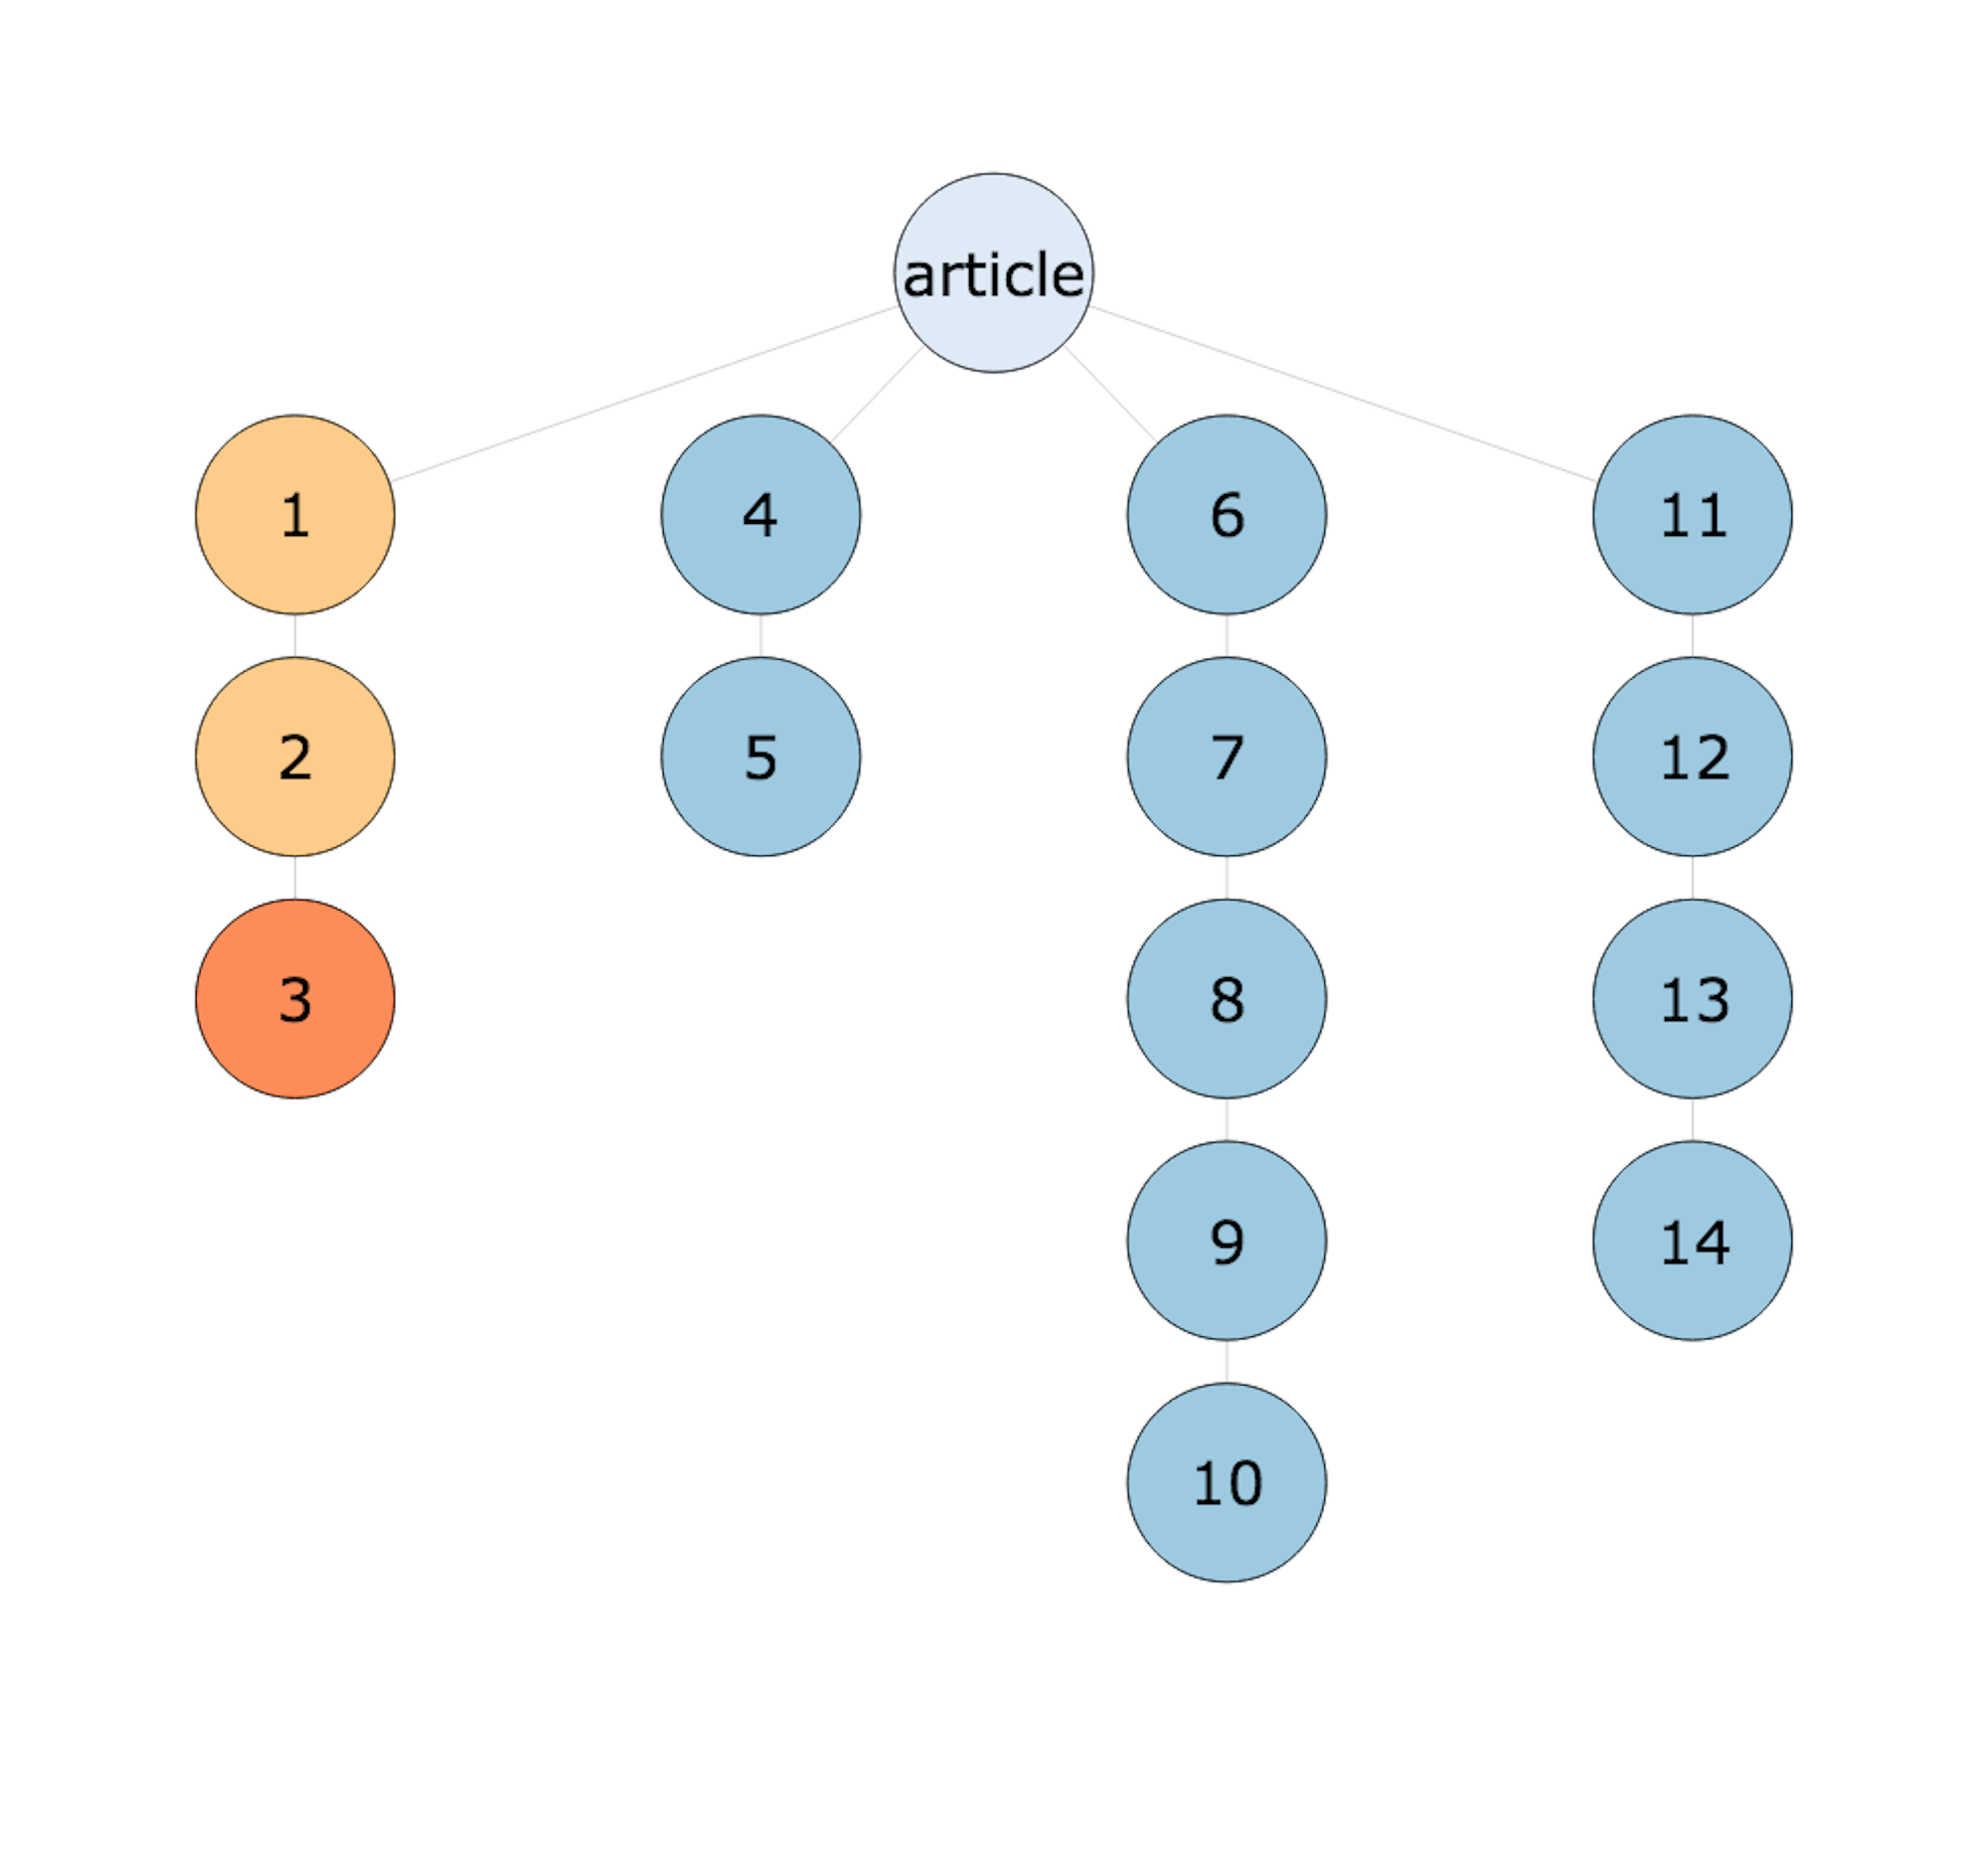
\includegraphics[width=0.5\textwidth]{images/approach/3.png} }}
    \subfloat[<t><c>\textbf{6}</c><c>\textbf{7}</c><c>\textbf{8}</c><c>\textbf{9}</c></t>]{{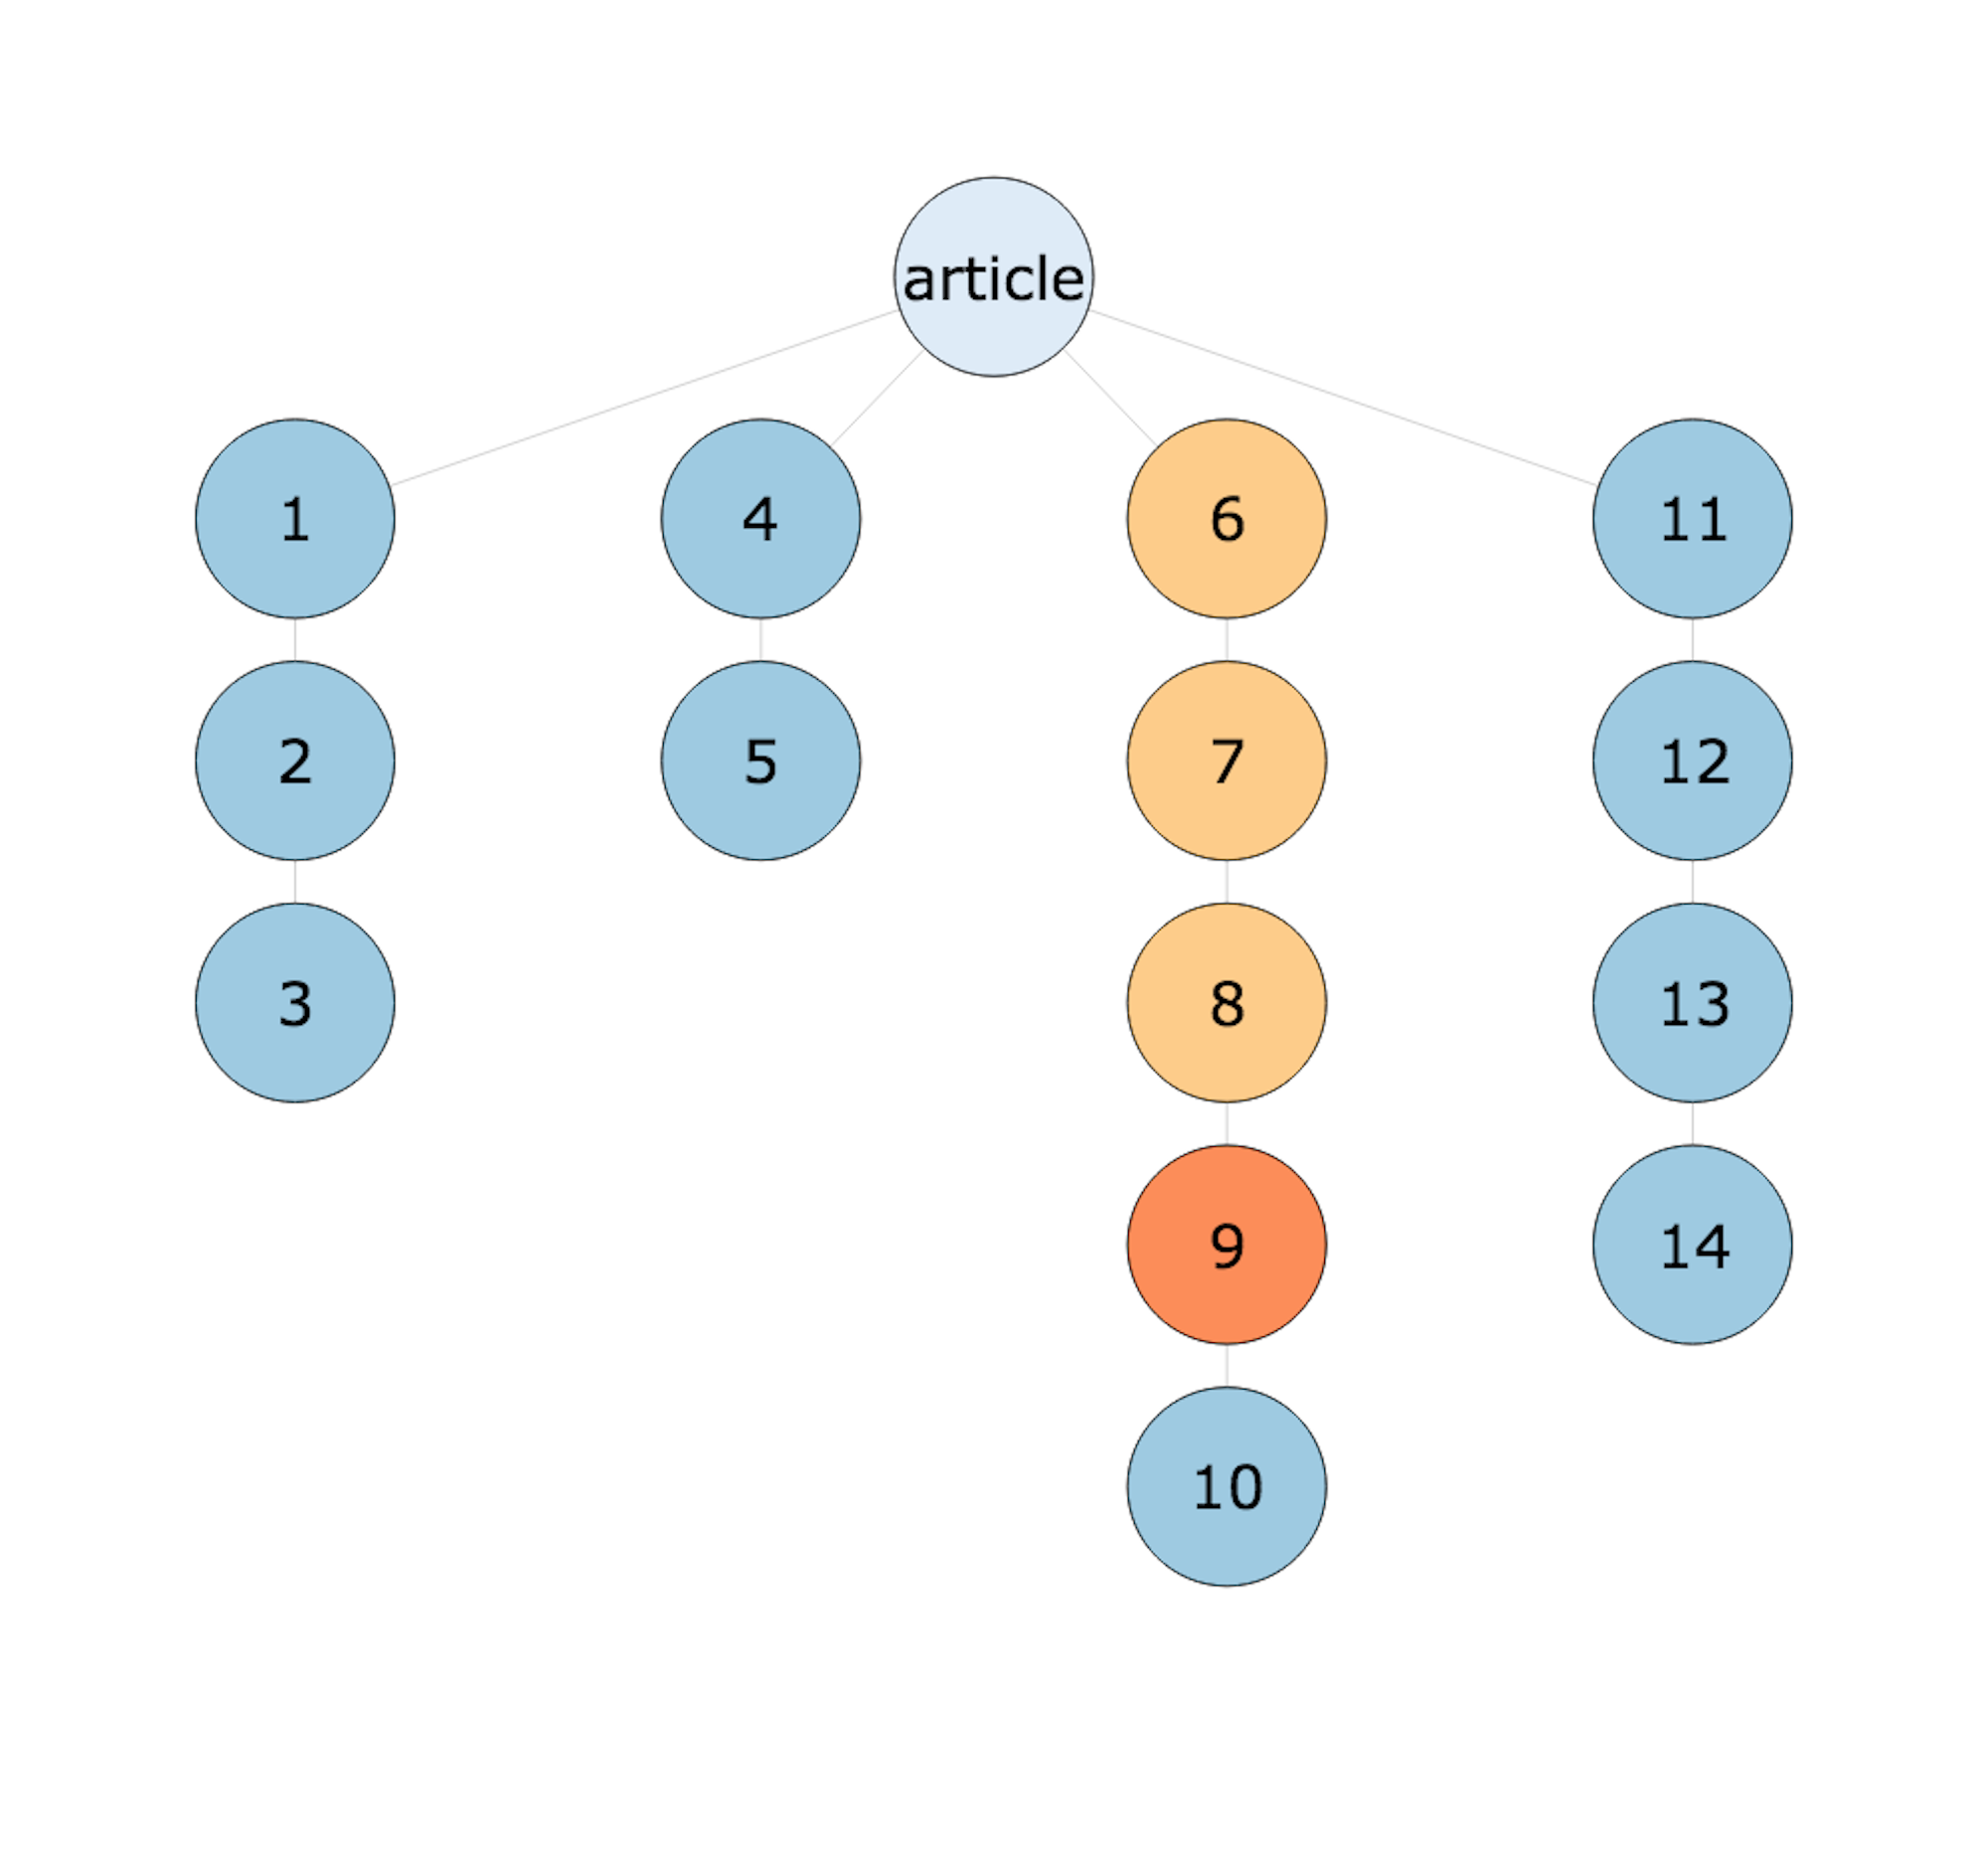
\includegraphics[width=0.5\textwidth]{images/approach/9.png} }}
    \caption{Prepending previous comments at the the example of Comment \textit{3} and Comment \textit{9}. Each comment is encapsulated by the special token (\textit{c}) to mark the start and end of a comment. Also a whole thread is indicated (\textit{t}).}
    \label{fig:approach_1}
\end{figure}

There exist different ways of how comment section appear on the Web.
We focus on sequential discussions where top-level comments appear directly under a news articles and other comments reply to them.
For each reply, we prepend the previous comments.
To separate the comments, we add special tokens between them.
This builds up a long chain of comments.
The comment with the corresponding annotation is always the last comment.
This is how the model can learn that the last comment in the chain is the comment to classify.
The previous comments only give additional information about the conversation.
Figure~\ref{fig:approach_1} illustrates the prepending for two comments. Comment~\textit{3} and Comment~\textit{9} are the samples to which the previous comments are prepended.
For Comment~\textit{3}, the final sequence is <t><c>1</c><c>2</c><c>3</c></t> and the original annotation of Comment~\textit{3} is attached to it.
The <c> and </c> represent the start and the end of comment respectively. Likewise <t> and </t> represent the start and the end of a discussion threads (or sub-dialogue).
To accomplish this, one has to iterate over all comments. % O(n)
Then for each comment, one has to gather all comments that are on the way to the parent node up to the root note -- the news article. %O(n)
This results in a complexity of $\mathcal{O}(n^2)$ for the algorithm.%see above: it's O(n^2), isn't it?

\newpage
In addition, the article's text and headline can be prepended to top-level comments.
There are some variations on how and when top-level comments are enriched.
First, there it is up to debate what kind of information about the article is given the model.
The article comprises headline, abstract, and the whole text.
Also some meta-information such as topic or date of publication are provided.
Second, it has to be decided whether to always add information about an article or only top-level comments.
To illustrate this with an example of the already mentioned Comment~\textit{3}, one could add information before the first comment like so: <t>article<c>1</c><c>2</c><c>3</c></t>.
This has one disadvantage.
Since multiples comments belong to one article, possibly thousands of comments, the article is duplicated in all the training samples.
This may lead to overfitting on the article information such as the title.
So the other idea is to not add article's information to Comment~\textit{3} and only to top-level comments.
For Comment ~\textit{1}, this results in following encoding: <t>article<c>1</c></t>.
The top-level comments do not have any previous comment so no comments can be prepended.
Without article information, there would not be any improvement over conversation-agnostic models for them.

With these adaption, there are potential problems.
Threads with a lot of comments result in duplication of some comments that appear early on in the discussion.
However, in practice internal memory is limited so the samples have to be truncated anyhow.
So here it is important to only truncate from the back to prevent losing valuable information of the last comment (with the annotation).
So for example only choose the last 1000 tokens of a comment chain.
But when cutting the chain on a token basis, it is likely that comments gets cut right in the middle.
This is why there are tokens to indicate the start and end of a comment.
The model is aware that the beginning of a chain is only a remainder of a previous comment.
This way of truncating on a token basis is superior to truncate on a comment basis.
One could think to only consider the previous N comments.
This would as well keep the length of each sample reasonable.
But comments vary in length (see Figure~\ref{fig:len_com}) and thus the sheer number of comments is not a guarantor for information.
The general idea to give as much information as possible to the model and let it decide which information is useful and which not.

So far, we only considered the sequential structure of news comment. Unlike with discussions on social media on Reddit or Twitter, there is often no nesting of replies. \textit{Prepend Previous} focuses on these sequential forms of discussions.
However, it can easily be adapted to to work for tree-like discussion structures.
Again, one has to iterate over all comments and go up the tree until the root.
This is visualized in Figure~\ref{fig:appr_tree_pp}.
In this case, the comments chains may have to be truncated more aggressively since it can happen that a comment appear in various sequences.
Overfitting on those comment is likely when fine-tuning a language model.
However, since there should be no fundamental difference between comments appearing earlier and later in a discussion, the language model should still be able to learn the languages of news comments.
Even if it sees comments appearing early in a discussion tree more often.

\begin{figure}
  \begin{center}
    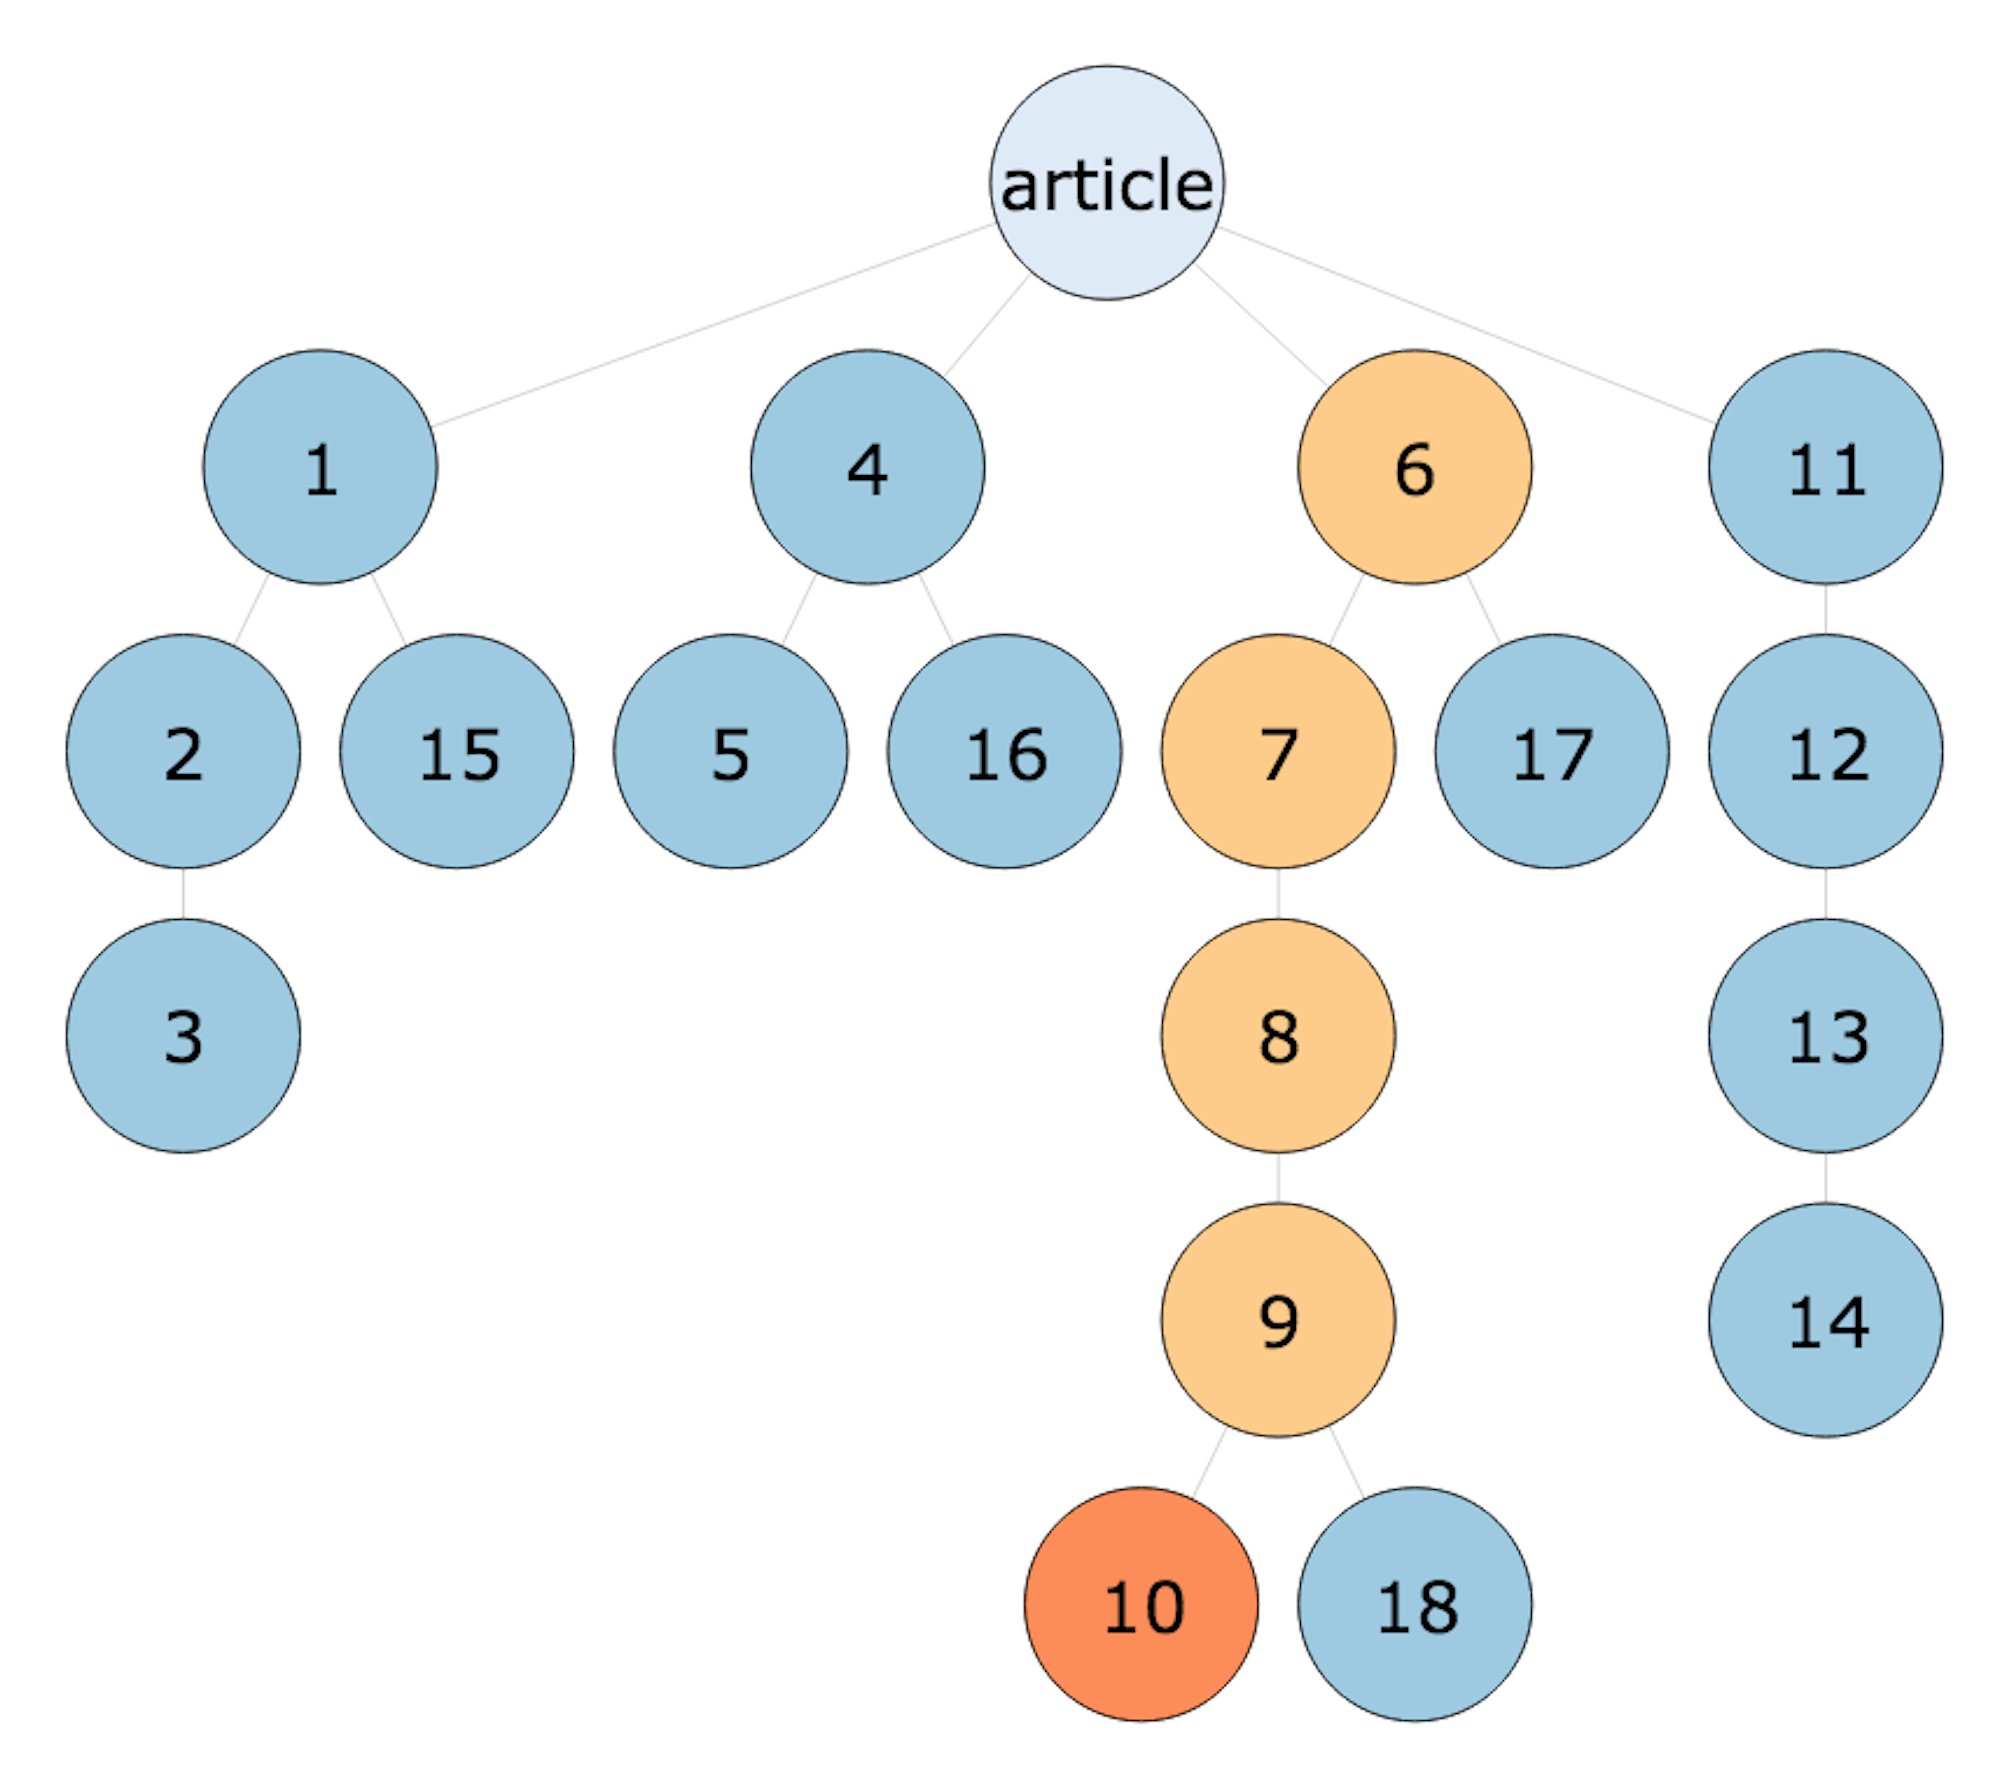
\includegraphics[width=0.5\textwidth]{images/approach/tree_10.png}
  \end{center}
  \caption{Prepending comments for tree-like comment structures is equivalent. The resulting sequence for Comment \textit{10} is: <t><c>\textbf{6}</c><c>\textbf{7}</c><c>\textbf{8}</c><c>\textbf{9}</c> <c>\textbf{10}</c></t>}
   \label{fig:appr_tree_pp}
\end{figure}

We implemented\footnote{\url{https://github.com/jfilter/masters-thesis}} the preprocessing in Python with Pandas\footnote{\url{https://pandas.pydata.org}} and Dask\footnote{\url{https://dask.org}}.
For the language model we used ULMFIT.
However, it can be applied to any other language-model-based text classification method because the preprocessing remains the same.
Recurrent neural network such as LSTMs are especially powerful since last internal state of the LSTM is used for classification. The comment to classify is always the last comment in a chain.

\section{ULMFIT for German}
\label{sec:ulmfit_for_de}

A general language model is required for using ULMFIT for text classification.
Since there does not exists a German pre-trained language model, we create one. Only with it, can we classify German comments of OMPC.

There has been effort to adapt ULMFIT to German but to no avail~\cite{ulmfit-germeval18}.
A first requirement is the existence of long, high-quality German texts.
It is important that the texts are long in order to learn long-term dependencies.
This allows the language model to get a deeper understanding of German.
We use a dump\footnote{\url{https://dumps.wikimedia.org}} of the entire German Wikipedia and extract the article's text with WikiExtractor\footnote{\url{https://github.com/attardi/wikiextractor}}.
To gather more data, we use news articles\footnote{In regard to ethical considerations, we note that we do not have the consent of the journalists who wrote the articles. However, journalists work in commission of a newspaper and no private information is attached to an article. And unlike for news comments, journalists know that their articles get processed automatically by, i.e., search engines.}.
We crawl news articles with News-Please\footnote{\url{https://github.com/fhamborg/news-please}} from several regional and national German newspaper.
Only documents with a length of at least 500 characters are kept.
The result is a collection of $3.278.657$ documents with altogether $1.197.060.244$ tokens. Compared to English, German is highly inflective.
And the language allows the construction of endless combination of compound nouns.
So a simple word-based approach would result in a large vocabulary.
It is encouraged to keep the vocabulary small, because in the last layer in a neural language model, a softmax activation function is computed over each entry in the vocabulary.
This is computationally intensive and a small vocabulary greatly speeds up the training process.
One way to do it, is to split words into sub-word units.
For instance, Byte-Pair Encoding (BPE) by Sennrich~et~al.~\cite{P16-1162} achieves this.
This is a compromise between word-based and character-based approaches.
The size of the vocabulary of sub-word units is fixed.
So the size of sub-units depend on the vocabulary size.
The smaller the vocabulary, the shorter the sub-word units.
Czapla~et~al.~\cite{czapla2018universal} successfully applied BPE to ULMFIT for Polish.
Since the splitting of word in sub-words is a model (or embedding) on its own, we can use a pre-trained model.
Heinzerling and Strube~\cite{heinzerling2018bpemb} provide pre-trained sub-word models\footnote{\url{https://nlp.h-its.org/bpemb}} for 275 languages.
The authors provide models for the vocabulary size from $1.000$ to $200.000$.
For Polish, Czapla et al. achieved the best results with vocabulary of $20.000$.
Since Polish and German are both Indo-Germanic languages, a parameter in the similar range should apply for German as well.
We choose a the German model with fixed vocabulary size of $25.000$.

\newpage

It follows an example of how it breaks up the German sentence
\begin{quote}
 ``\textit{Zeitungskommentare sind eine hervorragende M\"oglichkeit zum Meinungsaustausch}''
 \end{quote}
 into sub-word units:

\begin{quote}
	[`\_zeitungs',
 `komment',
 `are',
 `\_sind',
 `\_eine',
 `\_hervor',
 `ragende',
 `\_m\"oglichkeit',
 `\_zum',
 `\_meinungs',
 `austausch',
  '.']
\end{quote}

For instance, the German composite noun \textit{Meinungsaustausch} is split into two sub-word units. The white space is replaced with a special underscore token. We have to follow the preprocessing steps of the pre-trained model. This includes that all text is lowercased and all digits are replaced by a 0.

To train it, we take the default configuration of the English language:
an embedding size of 400 and 3 layered LSTM with 1150 hidden activations per layer.
But we fully disable dropout.
The amount of data is large enough such thats a strong regularization is not needed.
We trained for five epochs which took three days on a single GTX1800ti, with a batch size of $128$. The learning rate is chosen automatically by the learning rate finder ($0.00744..$). The training curves are in Figure~\ref{fig:germanlm} and the final model achieves a perplexity of $33.88..$. The language model is published for further usage\footnote{\url{https://johannesfilter.com/ulmfit-for-german}}.

 \begin{figure}
  \begin{center}
    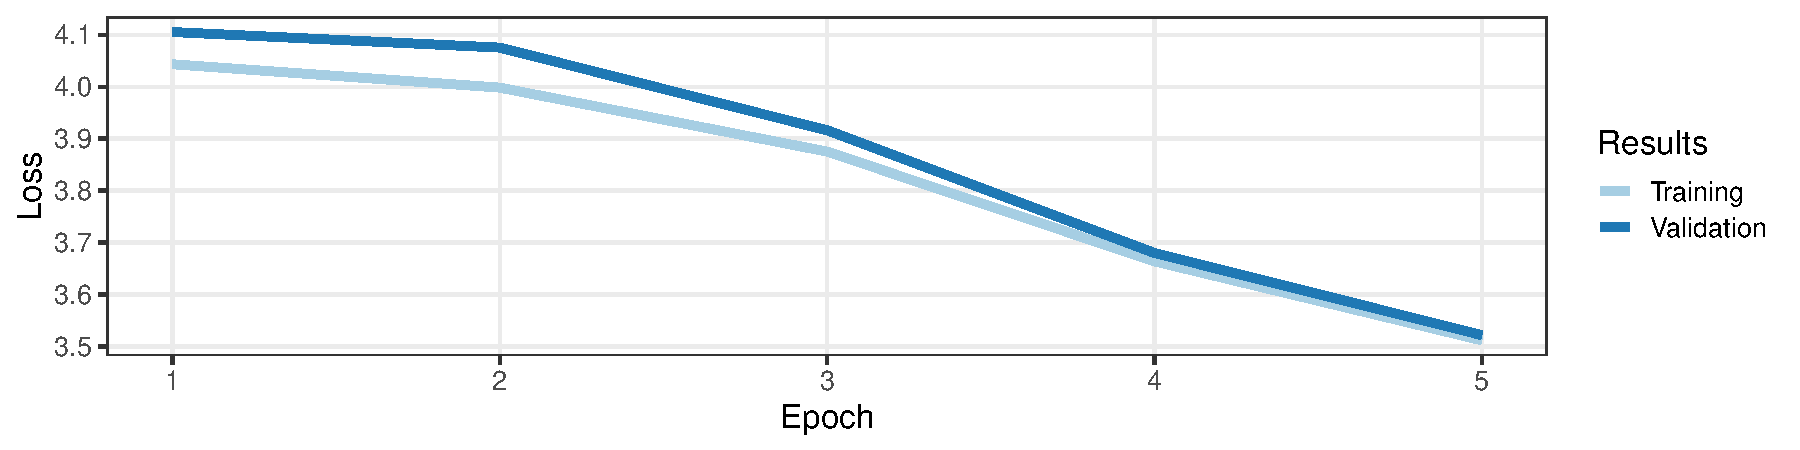
\includegraphics[width=\textwidth]{graphs/experiments/german_lm}
  \end{center}
	\caption{Training curves of the German language model.}
   \label{fig:germanlm}
\end{figure}
